\chapter{CoAP} \label{CoAP}

\section{Wat is CoAP?}

CoAP is een web transfer protocol speciaal ontwikkeld voor netwerkcomponenten die beperkt zijn in zowel geheugen als energieverbruik, als in machine-to-machine (M2M)\nomenclature{M2M}{Machine-to-machine}communicatie. Met M2M-communciatie bedoelen we communciatie tussen machines waar geen menselijke tussenkomst nodig is. Zoals de berichten die routers naar mekaar sturen om hun routingtabel te synchroniseren. Naast het minimaliseren van overhead concentreert CoAP zich ook op het automatiseren van taken. Het mechanisme van resource discovery (Zie paragraaf \ref{resourceDiscovery}) is hier een voorbeeld van. Met het verminderen van energieverbruik in het achterhoofd biedt CoAP naast synchrone ook asynchrone communicatie aan. Het biedt ook nieuwe soorten berichten aan zoals non-confirmable, piggy-backed, etc. Deze worden toegelicht in paragraaf \ref{betrouwbaarheid}\\


Het interactiemodel van CoAP is vergelijkbaar met het client/server model van HTTP. Hoewel, bij een CoAP implementatie voor M2M interacties kan een device bij de ene berichtuitwisseling client zijn, en bij de andere server. Een CoAP request is equivalent aan een HTTP request en wordt ook gestuurd van de client naar de server om een actie aan te vragen op een resource die zich op die server bevindt. De actie wordt bepaald door een method code (GET, PUT, POST of DELETE) en de resource wordt aangeduid met een Uniform Resource Identifier (URI).\nomenclature{URI}{Uniform Resource Identifier} De server antwoordt met een response die onder andere een response code bevat.\\

Verschillend met HTTP, gebeurt de berichtenuitwisseling asynchroon over een datagram-ge\"{o}ri\"{e}nteerd transport. Dit houdt in dat berichten mogelijks verloren gaan of in een andere volgorde kunnen aankomen dan dat ze verzonden zijn. Toch voorziet CoAP enige vorm van betrouwbaarheid met een soort bericht dat kan worden bevestigd door een acknowledgement (zie paragraaf \ref{betrouwbaarheid}). Wanneer zo'n bericht niet wordt bevestigd, wordt het bericht meermaals opnieuw gestuurd volgens het exponential back-off mechanisme (Zie paragraaf \ref{exponentialBackoff}).

CoAP definieert vier soorten berichten: Confirmable, Non-confirmable, Acknowledgement en Reset. Door gebruik te maken van method codes en response codes transporteren sommige van deze berichten requests of responses. In paragraaf \ref{communicatieMogelijkheden} gaan we hier dieper op in.\\

\begin{wrapfigure}{r}{0.5\textwidth}
\vspace{-10pt}
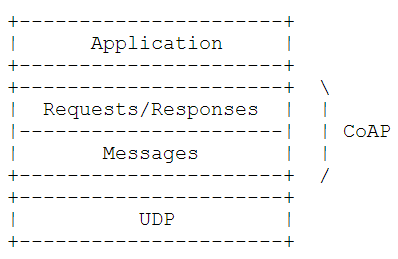
\includegraphics[width=0.5\textwidth]{fig/CoAPLaag}
\vspace{-30pt}
\caption{CoAP lagen (CoAP 14 draft)}
\vspace{-5pt}
\label{fig:CoAPLaag}
\end{wrapfigure}
We kunnen CoAP ook in het Open Systems Interconnection (OSI) -model \nomenclature{OSI}{Open Systems Interconnection} met 7 lagen plaatsen. Logisch gezien hebben we een CoAP berichtenlaag die het UDP gedeelte en de asynchroniteit van de berichten afhandelt en een request/response laag die gebruik maakt van method en response codes (zie Figuur~\ref{fig:CoAPLaag}). Nochtans bestaat CoAP in werkelijkheid slechts uit \'{e}\'{e}n laag waarbij berichtenuitwisseling en het request/response-mechanisme enkel en alleen door manipulatie van de header verwezenlijkt wordt.

\subsection{Berichtformaat}

\begin{wrapfigure}{r}{0.7\textwidth}
\vspace{-20pt}
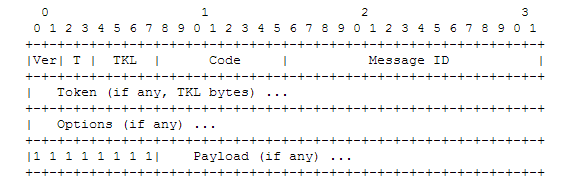
\includegraphics[width=0.7\textwidth]{fig/CoAPMessageFormat}
\vspace{-30pt}
\caption{Berichtformaat (CoAP 14 draft)}
\vspace{-10pt}
\label{fig:CoAPMessageFormat}
\end{wrapfigure}
Om een minimale overhead te realiseren worden de berichten zeer compact gehouden. We geven een kort overzicht van de onderdelen van het berichtformaat (zie Figuur~\ref{fig:CoAPMessageFormat}) en bespreken dan de belangrijke delen apart in subparagrafen. De eerste vier bytes stellen de header voor. Bemerk dus dat de header gerealiseerd wordt met slechts 4 bytes. Het veld na de header is optioneel en bevat een token waarvan de lengte aangegeven is in de header. Vervolgens zitten er nul of meer opties in het bericht.
Het laatste onderdeel van een bericht is de payload. Indien er een payload aanwezig is in het bericht, wordt die altijd voorafgegaan door een vaste byte, de payload marker (0xFF). Deze geeft het einde van de opties en het begin van de payload aan. Indien er geen payload is mag deze marker niet aanwezig zijn.

We merken hier op dat een token, opties en een payload optioneel zijn. Dit zorgt ervoor dat sommige berichten beperkt blijven tot de header van 4 bytes, wat zeer weinig is.

\subsubsection{Header}

Deze vier bytes worden opgedeeld in drie delen:
\begin{itemize}
\item Versiegetal (Ver): een 2-bit unsigned integer die de CoAP versie aangeeft. 
\item Type-aanduiding (T): een 2-bit unsigned integer die het berichttype aangeeft. De mogelijkheden zijn: Confirmable (CON) \nomenclature{CON}{Confirmable CoAP message} (0), Non-confirmable (NON)) \nomenclature{NON}{Non-Confirmable CoAP message} (1), Acknowledgement (ACK) \nomenclature{ACK}{Acknowledgement CoAP message} (2) of Reset (RST) \nomenclature{RST}{Reset CoAP message} (3).
\item Tokenlengte (TKL)\nomenclature{TKL}{ToKen Length}: een 4-bit unsigned integer die de variabele tokenlengte aangeeft.
\item Code: 8-bit unsigned integer die aangeeft of het bericht een request of een response overbrengt, of leeg is.
\item Message ID: een 16-bit unsigned integer die gebruikt wordt om duplicatie van berichten op te merken. Het wordt ook gebruikt om berichten van het type ACK/RST te linken aan berichten van het type CON/NON.
\end{itemize}

\subsubsection{Token}

Een token wordt gebruikt om een response te linken aan een request. De lengte wordt bepaald door de TKL en is nul tot acht bytes lang. Elk bericht heeft een token, dit kan lengte nul hebben. Wanneer een token nodig is, moet dat worden gegenereerd door de client. Indien de server wil dat zijn response geaccepteerd wordt, moet hij dit token zonder meer overnemen in zijn response.

\newpage

\subsubsection{Opties}

%\begin{wrapfigure}{r}{0.6\textwidth}
%\vspace{-20pt}
%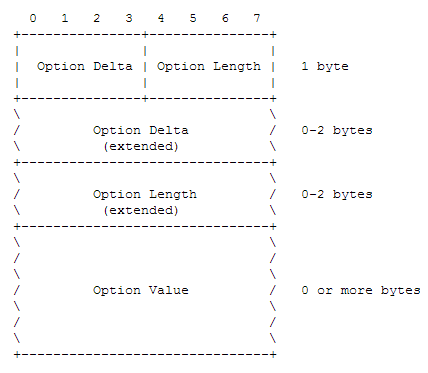
\includegraphics[width=0.6\textwidth]{fig/CoAPOpties}
%\vspace{-40pt}
%\caption{CoAP optie (CoAP 14 draft)}
%\vspace{-10pt}
%\label{fig:CoAPOpties}
%\end{wrapfigure}
Opties worden opgesteld door middel van de Type-Length-Value (TLV)\nomenclature{TLV}{Type Length Value} notatie (zie Figuur~\ref{fig:CoAPOpties}). Er wordt een mechanisme toegepast om opties in een pakket te stoppen, dat ervoor zorgt dat het pakket compact blijft en dus bijdraagt tot een minimale overhead.\\

Elke optie heeft een uniek nummer, maar wanneer meerdere opties in \'{e}\'{e}n pakket worden gestopt, worden de opties niet door dat nummer aangeduid, maar door de Option Delta. De Option Delta is het verschil tussen het nummer van een optie en dat van de vorige optie.
Concreet, stel dat men na een optie met nummer 6 een optie met nummer 11 wil plaatsen, dan wordt deze laatste aangeduid met Option Delta gelijk aan 5 (11 - 6). Dit alles samen maakt dat een minimale (lege, maar daarom niet nutteloze) optie slechts 1 byte in beslag neemt. Dit heeft als gevolg dat opties na elkaar moeten worden geplaatst met oplopende Option Numbers.\\

Indien de Option Delta 13 of meer is, schiet dit systeem tekort. Daarom zijn er speciale waarden ingevoerd die het gebruik van extended een extended Option Delta aangeven. Indien de Option Delta groter is dan 12, maar kleiner is dan 269, wordt als Option Delta waarde 13 gebruikt. Er wordt dan een extra byte voor de Option Value gezet dat opgevuld wordt met de echte Option Delta - 13. Indien de Option delta meer is dan 268, wordt als Option Delta de waarde 14 gebruikt. Deze waarde geeft aan dat er twee extra bytes gebruikt worden. Deze bytes worden opgevuld met de echte Option Delta - 269. De waarde 15 mag niet als Option Delta gebruikt worden want deze geeft het begin van de payload aan. Voor Option Length zijn de regels analoog.


\begin{figure}[h]
\centering
%\vspace{10pt}
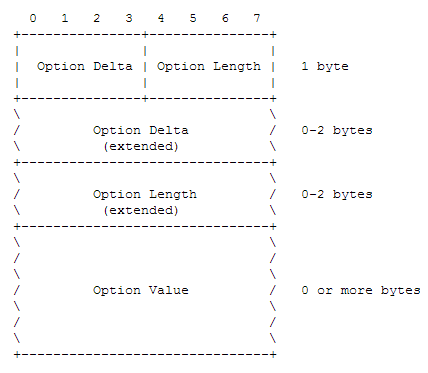
\includegraphics[width=0.6\textwidth]{fig/CoAPOpties}
\vspace{-10pt}
\caption{CoAP optie (CoAP draft 16)}
\label{fig:CoAPOpties}
\end{figure}

\newpage

\subsubsection{Verschil met HTTP}

Als we dit kort vergelijken met het berichtformaat van HTTP (zie Figuur~\ref{fig:HTTPMessageFormat}) zien we dat er aanzienlijke verschillen zijn. Bij HTTP zijn request en response niet helemaal gelijk. We kijken eerst naar de HTTP request.

Deze is opgedeeld in drie delen. Een requestlijn die op zijn beurt opgedeeld is in drie delen, gescheiden door een spatie. Het eerste deel is de methodenaam (GET, POST, HEAD, PUT of DELETE voor HTTP 1.1). Het tweede deel is de URL van de gevraagde resource en het laatste deel is het versienummer. Vervolgens zijn er een aantal headerlijnen die bijkomende opties voorstellen. De entity body wordt gebruikt door de POST methode om gegevens door te sturen en wordt gescheiden van de headerlijnen door een lege lijn. Bijkomend wordt elke lijn (ook de lege) afgesloten met een carriage return (CR)\nomenclature{CR}{Carriage Return} en een line feed (LF\nomenclature{LF}{Line Feed}).

De HTTP response is analoog aan de request met als verschillen dat de eerste lijn opgebouwd is uit het versienummer, de statuscode die aangeeft wat het resultaat van de request inhoudt en een korte beschrijving van de status code.\\
Het is dus duidelijk dat een HTTP bericht aanzienlijk groter zal zijn dan een CoAP bericht.

\begin{figure}[h]
\vspace{10pt}
\centering
\subcaptionbox{Request}
{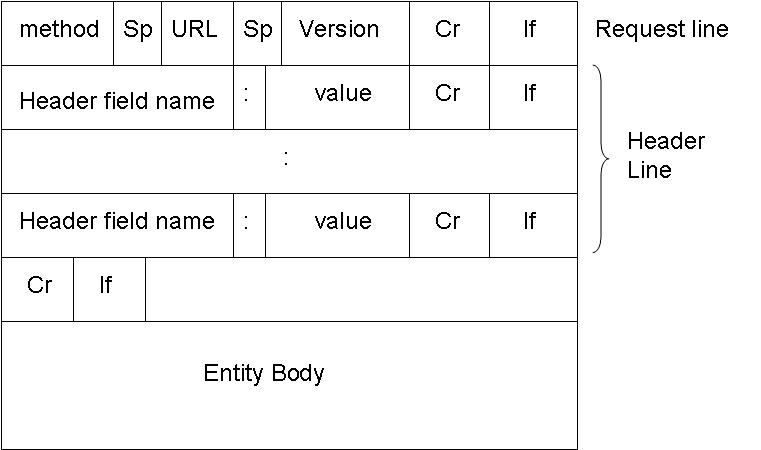
\includegraphics[width=0.45\textwidth]{fig/HTTPRequestMessageFormat}}
\subcaptionbox{Response}
{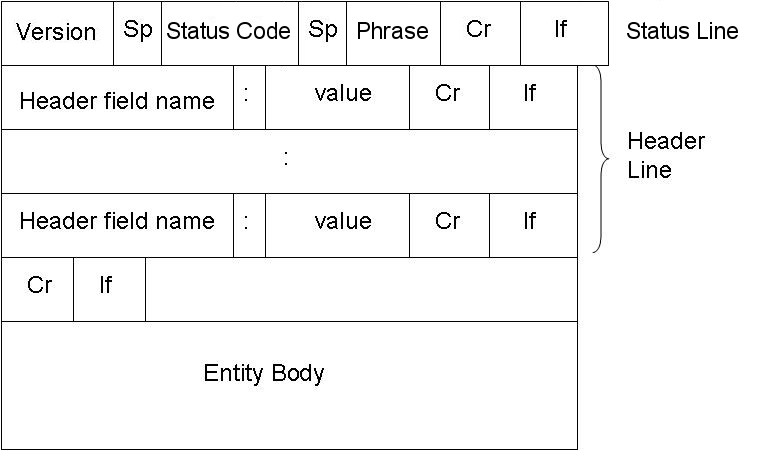
\includegraphics[width=0.45\textwidth]{fig/HTTPResponseMessageFormat}}
\caption{HTTP Message Format}\label{fig:HTTPMessageFormat}
\end{figure}

\newpage

\section{Communicatiemogelijkheden} \label{communicatieMogelijkheden}

In deze paragraaf bespreken we de communicatiemogelijkheden van CoAP. We bekijken de variabele betrouwbaarheid van CoAP berichten en gaan na hoe het request/response model bij CoAP werkt aan de hand van voorbeelden. Als laatste lichten we het principe van blockwise transfer even toe.

\subsection{Betrouwbaarheid} \label{betrouwbaarheid}

HTTP realiseert een betrouwbare en robuuste vorm van communicatie. Het is gebaseerd op het Transmission Control Protocol (TCP), dit protocol zet een verbinding op aan de hand van stream sockets. Het zorgt ervoor dat pakketten gegarandeerd aankomen bij de bestemming en dit in volgorde van verzending. Maar deze betrouwbaarheid komt met een prijs, namelijk extra netwerkbelasting voor het opzetten en beheren van die verbinding. In tegenstelling tot HTTP dat gebouwd is op TCP, is CoAP gebaseerd op berichtenuitwisseling over UDP. Wanneer men met dit protocol werkt, is er echter geen garantie dat pakketten aankomen en wanneer dat wel het geval is, kan de volgorde van aankomst gewijzigd zijn ten opzichte van verzending. Daarom moet men bij CoAP zelf de betrouwbaarheid verzorgen indien nodig.

\subsubsection{Confirmable berichten}

Wanneer we de betrouwbaarheid van de berichtenuitwisseling willen opdrijven, merken we de berichten als CON. Een CON-bericht moet door de server worden beantwoord met een ACK-bericht (zie Figuur~\ref{fig:berichtuitwisseling}), dit ACK-bericht moet hetzelfde message ID bevatten als het CON-bericht waarop geantwoord wordt. Wanneer CON-berichten niet worden beantwoord met een ACK-bericht v\'{o}\'{o}r een bepaalde timeout, wordt het bericht opnieuw verzonden. Bij het opnieuw verzenden wordt een exponential back-off mechanisme toegepast. Eerst wordt een timeout bepaald tussen een ACK\_TIMEOUT en ACK\_TIMEOUT x ACK\_RANDOM\_FACTOR, wanneer die timeout verstrijkt wordt het CON-bericht opnieuw verzonden en de timeout verdubbeld. Wanneer de server niet in staat is het CON-bericht te verwerken, wat betekent dat die zelfs geen geldige error response kan geven, antwoordt die met een RST-bericht in plaats van met een ACK-bericht.

\subsubsection{Non-confirmable berichten}

Soms heeft een bericht geen betrouwbaar transport nodig. Een voorbeeld hiervan is een stroom van sensordata waarbij elke meting verstuurd wordt met een NON-bericht. Dit soort berichten wordt niet bevestigd met een ACK bericht, maar de berichten hebben wel nog steeds een message id om duplicatie van berichten te detecteren (zie Figuur~\ref{fig:berichtuitwisseling}). Wanneer een ontvanger niet in staat is het bericht te verwerken, opnieuw bedoelen we daarmee dat het geen geldige error response kan geven, zendt die een RST-bericht naar de zender.

\begin{figure}[h]
\vspace{10pt}
\centering
\subcaptionbox{Confirmable}
{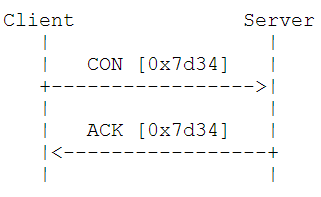
\includegraphics[width=0.3\textwidth]{fig/CoAPConfirmable}}
\hspace{30pt}
\subcaptionbox{Non-confirmable}
{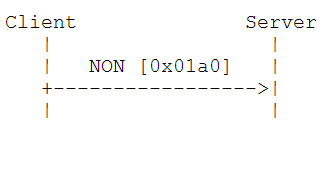
\includegraphics[width=0.3\textwidth]{fig/CoAPNonConfirmable}}
\caption{Berichtuitwisseling (CoAP 14 draft)}
\label{fig:berichtuitwisseling}
\end{figure}

\subsection{Request/response model}

\subsubsection{Piggy-backed response}

Wanneer een request met een CON bericht verstuurd wordt, is het mogelijk dat het antwoord meteen beschikbaar is bij de server. Indien dit het geval is, wordt het antwoord op de request meteen meegestuurd met het ACK bericht. Dit wordt een piggy-backed response genoemd. In Figuur~\ref{fig:CoAPPiggyBacked} worden twee voorbeelden van GET requests met piggy-backed responses getoond. De ene is succesvol, de andere geeft een error response terug.
\begin{figure}[h]
\vspace{10pt}
\centering
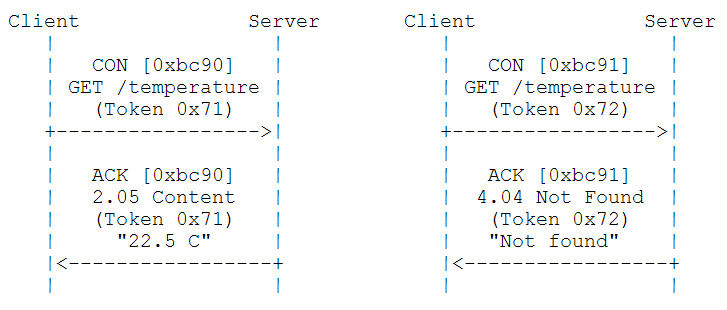
\includegraphics[width=0.7\textwidth]{fig/CoAPPiggyBacked}
%\vspace{-10pt}
\caption{Twee GET requests met piggy-backed responses (CoAP 14 draft)}
\label{fig:CoAPPiggyBacked}
\vspace{-20pt}
\end{figure}

\newpage

\subsubsection{Separate response} \label{separate}

\begin{wrapfigure}{r}{0.3\textwidth}
\vspace{-40pt}
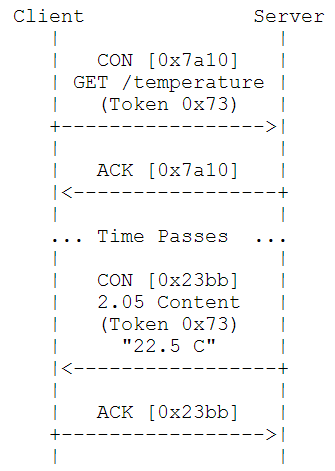
\includegraphics[width=0.3\textwidth]{fig/CoAPSeperateResponse}
\vspace{-30pt}
\caption{GET request met seperate response (CoAP 14 draft)}
\label{fig:SeparateResponse}
\vspace{-100pt}
\end{wrapfigure}
Wanneer de server niet onmiddellijk kan antwoorden op de request van de client, antwoordt die met een leeg ACK bericht zodat de client niet zou beginnen heruitzenden als gevolg van het exponential back-off mechanisme. Wanneer de response klaar is, stuurt de server dit antwoord in een nieuw CON bericht dat op zijn beurt beantwoord moet worden door de client. Dit soort van berichtenuitwisseling heet separate response (zie Figuur~\ref{fig:SeparateResponse}).
\\
\\
\\

\subsection{Blocks} \label{blocks}
CoAP werkt goed als de berichten geen of kleine payloads bezitten. Dit mag je veronderstellen als je werkt met temperatuursensors of lichtschakelaars. Maar soms is het nodig dat applicaties berichten sturen met grotere payloads, zoals bij resource discovery dat we in \ref{resourceDiscovery} bespreken of bij resources die nu eenmaal veel gegevens als antwoord op een request hebben.\\

Bij HTTP doet TCP al het werk om de pakketten te fragmenteren en ervoor te zorgen dat de deelpakketten in de juiste volgorde verwerkt worden. Dit is niet mogelijk bij CoAP aangezien UDP als transportprotocol gebruikt. Bij UDP zijn er ook verschillende niveau's van mogelijke fragmentatie, maar gebruik van deze niveau's moet vermeden worden om de fragmentatie af te handelen op applicatieniveau. Op deze manier worden meerdere blokken informatie van een enkele resource representation uitgewisseld via meerdere request-response paren. Belangrijk op te merken hierbij is dat elk request-response paar afzonderlijk af te handelen is door client en server. Dit heeft als gevolg dat er geen connectie opgezet moet worden en dat de server geen geheugen moet vrijmaken om bij te houden welk blok hij moet versturen. Welke de niveau's zijn en waarom er voor de Block Options gekozen is wordt uitvoerig besproken in de draft 'Blockwise transfers in CoAP' \cite{blockwiseTransfer}.

\subsubsection{Block Options}
Om grote payloads op een goede manier te ondersteunen worden twee Block Options ingevoerd. Optie 23 heeft als naam Block2 en geeft informatie over de request payload. Optie 27 heeft als naam Block1 en geeft informatie over de response payload. Beide opties  geven een blockwise transfer aan en kunnen zowel in requests als responses voorkomen. Ze ondersteunen blokgroottes die een macht van twee zijn, beginnend bij 16 t.e.m. 1024 bytes.

\subsubsection{Structuur}
Bij beide opties hebben de optiewaarden dezelfde structuur. De lengte van de waarde is variabel en kan 1, 2 of 3 bytes lang zijn zoals te zien in figuur~\ref{fig:blockOption}.
\begin{figure}[h]
\centering
\includegraphics[width=0.6\textwidth]{fig/blockOption}
\caption{Blokoptiewaarde - bytes en bits worden aangegeven bovenaan de figuur}
\label{fig:blockOption}
\end{figure}

\noindent
Wat we nog uit figuur~\ref{fig:blockOption} halen is dat het telkens drie elementen bevat:
\begin{enumerate}
\item NUM (Block Number): het relatief nummer van het blok binnen een sequentie van blokken.
\item M (More Flag): is dit het laatste blok in een reeks?
\item SZX (Size Exponent): geeft de grootte van het blok.
\end{enumerate}

\noindent
De blokgrootte is ge\"{e}ncodeerd gebruik makend van een drie-bit unsigned integer. 0 komt overeen met $ 2^{4} $ en 6 komt overeen met  $ 2^{10} $. Concreet wordt de grootte van het blok gegeven door  $ 2^{ SZX + 4} $. 7 mag niet gebruikt worden als waarde omdat deze gereserveerd is.

\section{Extra Features}

\subsection{Observe} \label{observe}

Wanneer een resource observable is of anders gezegd, de observe functionaliteit ondersteunt, kan die resource op eigen initiatief data sturen naar eventueel ge\"{i}nteresseerde clients. Een client kan zijn interesse uiten door een CON bericht te sturen naar de server dat een lege Observe Option (optie 6) bevat. Wanneer de client dan een ACK bericht terug krijgt met een observe option, weet die dat de server de client heeft toegevoegd aan de lijst van observers. Een client kan aangeven aan de server dat die niet meer ge\"{i}nteresseerd is door een RST bericht te sturen naar de server. De server verwijdert de client dan uit de lijst van ge\"{i}nteresseerden.

\subsection{Resource discovery} \label{resourceDiscovery}
Resource discovery zorgt ervoor dat lokale client en servers elkaar kunnen vinden en met elkaar kunnen interageren zonder menselijk tussenkomst.

\subsubsection{Principe}
\noindent
Resources kunnen maar aangesloten zijn op een device. Dit device maakt een fictieve resource aan met als naam de well-known/core. Deze fictieve resource bevat een opsomming van alle resources verbonden met dit device en een aantal gegevens over deze resources onder de vorm van attributen. Sommige well-known/core's bevatten ook verwijzingen naar resources op andere devices. Gebruikers kunnen een GET-request sturen om de well-known/core op te halen en hebben dan deze informatie tot hun beschikking. De well-known/core bevat echter veel informatie die niet in een enkel request-response paar uitgewisseld kan worden. Daarom wordt er gebruik gemaakt van blocks welke uitgelegd worden in \ref{blocks}. De manier waarop deze informatie doorgegeven wordt, is door gebruik te maken van het CoRE Link Format \cite{coapDiscovery}.

\subsubsection{CoRE Link Format}
Er worden geen resources opgeslaan in de well-known/core maar links naar deze resources. Als formaat van de links moet het CoRE Link Format gebruikt worden. Een resource wordt uniek ge\"{i}dentificeerd met een uri die tussen kleiner-dan (\textless) en een groter-dan (\textgreater) teken staat. Na de uri worden alle attributen opgesomd gescheiden door een puntkomma (;). De attributen zelf hebben de vorm van een name-value paar. Sommige attributen kunnen meerdere waarden hebben, deze waarden worden dan gescheiden door een spatie. Tot slot worden verschillende links gescheiden met een komma (,).\\

\noindent
Als voorbeeld geven we het antwoord op een GET-request van een well-known/core:\\
\textless/temp\textgreater;rt="temperature-c";if="sensor",\\
\textless/light\textgreater;rt="light-lux";if="sensor"\\
We zien dat het device met deze core twee resources aanbiedt. De eerste resource wordt ge\"{i}dentificeerd met de uri /temp, de andere met /light. Beide resources hebben twee attributen maar er zijn meer attributen mogelijk. We sommen de meest voorkomende attributen op:
\begin{itemize}
\item obs (Observable): Geef aan of de resouce observable is, indien deze optie ontbreekt wordt aangenomen dat de resource niet observable is.
\item rt (Resource Type): Geeft het type van de resource. De waarden zijn afhankelijk van de gebruikte applicatie. Ze hebben als nut dat binnen een applicatie, resources van hetzelfde type herkent kunnen worden. Dan kan via query filtering, alle resources van een type opgehaald worden.
\item ct (Content Type): Bevat een opsomming van de content formats die ondersteund worden door deze resource. 
\item if (Interface Description): Bevat een beschrijving van welke methoden deze resource ondersteunt.
\item sz (Maximum Size Estimate): Geeft aan hoe groot het maximum aantal gegevens ongeveer is als antwoord op een GET-request.
\item title: Bevat een omschrijving van deze resource.
\item anchor: 
\item rel: 
\end{itemize}
De lijst met alle attributen vind je in de CoRE Link Format draft \cite{coapDiscovery}.

\subsubsection{Core ophalen}
Om een well-known/core op te halen, moet je twee maal de Uri-Path Option (optie 11) toevoegen aan een GET-request die gericht is naar het IP-adres van het device waar de core zich op bevindt. De eerste keer met als value 'well-known' en de tweede keer gebruik je als value 'core'.\\

We bespreken een voorbeeld om de lezer 

\subsubsection{Query Filtering}
Het is mogelijk een specifieke discovery uit te voeren indien er enkel informatie over één resource moet gekend zijn of enkel de resources waarbij een bepaald attribuut een specifieke waarde heeft. Dit heeft als voordeel dat het netwerk niet overbodig belast moet worden als dat niet nodig is. De query-filter wordt voorgesteld door een name-value pair. Deze wordt toegevoegd door de Uri-Query Option (optie 15) te gebruiken.

